\documentclass[10pt, conference, compsocconf]{IEEEtran}
\hyphenation{op-tical net-works semi-conduc-tor}

\usepackage{cite}
\usepackage{epsfig}
\usepackage{graphicx}
\usepackage{subfigure}
\usepackage{algorithmic}

\begin{document}
\bibliographystyle{IEEEtran}

%\title{Online Training Machine Learning based Decision Maker for Mobile
%Offloading Framework}
\title{Machine Learning-based Mobile Offloading Scheduler with Online
Training}


\author{\IEEEauthorblockN{Heungsik Eom, Renato Figueiredo}
\IEEEauthorblockA{Advanced Computing and Information Systems Laboratory\\
Electrical and Computer Engineering\\
University of Florida, Gainesville, Florida, USA\\
\{hseom, renato\}@acis.ufl.edu}
\and
\IEEEauthorblockN{Huaqian Cai, Gang Huang}
\IEEEauthorblockA{Operating System and Middleware Laboratory\\
School of Electronics Engineering and Computer Science\\
Peking University, Beijing, China\\
\{caihq12, hg\}@pku.edu.cn}
}

\maketitle

\begin{abstract}
%
%OpenCL has emerged as the open standard for parallel programming for
%heterogeneous platforms enabling a uniform framework to discover,
%program, and distribute parallel workloads to the diverse set of compute
%units in the hardware.
%
%For that reason, there have been efforts exploring the advantages of
%parallelism from the OpenCL framework by offloading GPGPU workloads
%within an HPC cluster environment.
%
%In this paper, we present an OpenCL-based remote offloading framework
%designed for mobile platforms by shifting the motivation and
%advantages of using the OpenCL framework for the HPC cluster environment
%into mobile cloud computing where OpenCL workloads can be exported from
%a mobile node to the cloud.
%
%Furthermore, our offloading framework handles service discovery, access
%control, and data privacy by building the framework on top of a social
%peer-to-peer virtual private network, SocialVPN. 
%
%We developed a prototype implementation and deployed it into local- and
%wide-area environments to evaluate the performance improvement and
%energy implications of the proposed offloading framework.
%
%Our results show that, depending on the complexity of the workload and
%the amount of data transfer, the proposed architecture can achieve more
%energy efficient performance by offloading than executing locally.
\end{abstract}

\begin{IEEEkeywords}
Mobile platform, computation offloading, machine learning, runtime
scheduler, online training
\end{IEEEkeywords}

\section{Introduction}
%
Over the last decade, mobile offloading techniques have emerged as
intelligent means to overcome the constraints of the limited resources
from mobile platforms, smartphones and tabletPCs, so that these types of
devices delegate computationally intensive computing tasks to more
powerful external resources such as personal workstations or cloud
servers.
%
Initially, most of research interests on mobile offloading techniques
have focused on core mechanisms in which \textit{what to offload} and
\textit{how to offload} have been primarily considered. 
%
The research community has studied various approaches to implement mobile
offloading frameworks which fall in the following categories:
application partitioning~\cite{spectra, maui, cuckoo}, thread
migration~\cite{clonecloud, comet}, application migration~\cite{hung},
and distributed offloading frameworks~\cite{mmr, sonora, serendipity}.\\
%
\indent However, one important fact from an offloading performance
standpoint of view is that benefits from offloading
computation-intensive portions of mobile applications can be influenced
by various internal and external factors such as application
requirements, network conditions, and computing capabilities of mobile
or external devices.
%
Thus, \textit{whether to offload or execute locally} needs to be
decided periodically by monitoring aforementioned dynamic features on
runtime.
%
Otherwise, incorrect offloading decisions may cause the performance
degradation or worse energy consumption.
%
For that reason, research focuses have been naturally shifted into
dynamic scheduling or decision making problems for mobile offloading
framework.
%
For example, Kwon et al.~\cite{kwon} consider a simple rule-based
scheduler in which the framework decides to offload the mobile
computation only when the data transfer size is higher than a certain
threshold.
%
MAUI~\cite{maui} utilizes a linear regression model among predefined
features to make offloading decisions.\\
%
\indent Even though these studies on the runtime scheduler for mobile
offloading system take dynamic features such as data transfer size or
network conditions into account to make offloading decisions, it is
impractical for these approaches to build a globally well-defined
offloading decision policy while considering all possible cases against
dynamic mobile environments.
%
Furthermore, it is difficult to generalize the above efforts for various
mobile application use case scenario, since different applications need
to have different offloading decision policies due to different
application requirements or characteristics.
%
Therefore, in practice, it is necessary for the scheduler to learn
from self-observation of the previous decision correctness and to
dynamically adapt the decision policy on runtime, thereby an identical
decision model can be \textit{generally} applied to various mobile
applications without any predefined decision policies.\\
%
\indent In this paper, we aim to develop a general framework for a
runtime adaptive scheduler for mobile offloading framework by
employing various types of machine learning techniques.
%
By applying machine learning techniques to scheduling problems
for mobile offloading framework, the machine learning classifier can
make decisions on whether mobile computations should be offloaded to
external resources or executed locally.
%
To this end, we modularized our previous work on the machine
learning-based runtime scheduler~\cite{ml} in which any appropriate
machine learning classifiers can be utilized for the runtime scheduler
for mobile offloading framework.
%
This work can be plugged and played with any types of mobile offloading
frameworks in conjunction with the well-defined APIs to monitor and
acquire dynamic features such as data size, network conditions, or the
status of external devices. 
%
Furthermore, our work supports an online training mechanism for
the machine learning-based runtime scheduler such that it learns from
observation on the previous offloading decision performance, and
dynamically adapts its decision policy on runtime.\\
%
\indent As part of the modularization effort, we integrated the
modules of the machine learning-based runtime scheduler into the Java-based
offloading-capable mobile applications which are automatically
refactored by a novel tool, called \textit{DPartner}.
%
Originally, the offloading-capable mobile applications regenerated by
DPartner depend on the web based user interface to offload or execute
the offloadable computing tasks (i.e. classes) in local, so the user
schedules them manually by manipulating the UI in a drag-and-drop way.  
%
By combining the machine learning-based runtime scheduler with these
applications, the user can be free of the burden of the scheduling
tasks.
%
Based on this integration, we evaluated the cost and performance for
three machine learning algorithms, instance based learning, perceptron,
and na\"{i}ve bayes with respect to classifier build time,
classification time, and scheduling accuracy.
%
Even though there have been prior related studies which suggest
utilizing machine learning techniques for mobile computing environments,
to the best of our knowledge, our work is the first to consider the
online training mechanism for the machine learning-based runtime
scheduler for mobile offloading framework and demonstrate the
performance and cost of various machine learning algorithms for the use
of the runtime scheduler of mobile offloading framework.\\   
%
\indent The rest of the paper is organized  as follows.
%
In Section II, we overview prior research efforts on offloading decision
problems in mobile offloading framework as well as the use of machine
learning techniques for scheduling problems from various domains.
%
Section III summarizes our previous work which proposed the machine
learning based runtime scheduler for mobile offloading framework.
%
Section IV motives the concept of the online machine learning-based
runtime scheduler.
%
In Section IV and V, we explain and evaluate our implementation of the
online ML scheduler.
%
Also, Section VI describes the current and potential applications for
our work.
%
Finally, we conclude the paper in Section VII.
%
\section{Related Works}
%
\section{Runtime Scheduler for Mobile Offloading System}
%
In this section, we summarize our previous work on the machine
learning-based runtime scheduler for mobile offloading framework.
%
In our previous work, we noticed the offloading performance dependency on
various dynamic features such as data size and network conditions.
%
Then, we suggested applying machine learning techniques to the runtime
scheduler for mobile offloading framework by showing the performance and
cost among various machine learning algorithms. 
% 
\subsection{Offloading Performance}
%
In our previous work~\cite{ml}, we validated the necessity and efficacy
of the runtime scheduler for mobile offloading framework through
detailed measurement experiments.
%
With the OpenCL-based mobile offloading framework~\cite{ocloff}, we
performed various experiments using four different OpenCL workload
kernels used in a variety of areas such as image processing filters and
mathematical simulations.
%
Also, in order to observe the impact of different network conditions on
the offoading performance, we configured different network conditions:
local area network, campus network, and wide area network (i.e. Amazon
EC2 cloud).
%
In the evaluation, we verified that different network conditions cause
significantly different offloading performance.
%
In most cases, offloading to the remote resource located in local area
network has better performance than local processing in four OpenCL
workload kernels used for the experiments.
%
In contrast, offloading to the remote resource located in campus network
and Amazon EC2 cloud, where have much limited network conditions than
local area network, can exhibit longer execution time than local
processing according to the size of data transfer.\\ 
%
\indent It is worth noting that each OpenCL workload kernel shows
the different performance, even though they process the similar size of
data.
%
This is because each kernel has different computational complexities so
they gain the different amount of performance improvement while paying
the same cost to send the data to the remote resource.
%
These results show that there exists the offloading performance
variation over different network conditions and OpenCL workload kernels.
%
Consequently, proper scheduling can have a significant impact on the
offloading performance, and mobile offloading framework requires the
support from the runtime scheduler.
%
\subsection{Machine Learning-based Runtime Scheduler}
%
Based on our observation, we applied machine learning techniqeus to the
runtime scheduling problem for mobile offloading framework.
%
For doing this, we first chose a set of relevant attributes which have
an impact on making offloading decisions.
%
Also, by running the OpenCL-based offloading framework with different
network configurations, OpenCL workload kernels, and data size, we
collected a total 640 data instances to train and test the classifiers
of various machine learning algorithms.
%
Using the gathered dataset, we trained various machine learning
classifiers with \textit{Weka}, a Java-based open source package for
machine learning techniques.
%
Finally, we implemented the machine learning-based runtime scheduler by
building the trained machine learning classifiers onto the
OpenCL-based mobile offloading system.\\
%
\indent In order to evaluate the machine learning-based runtime
scheduler for mobile offloading framework, we deployed the OpenCL-based
offloading system under various network bandwidth controlled by a
network characteristic tool called \textit{Traffic Control} (TC).
%
In our evaluation, we observed that most of the machine learning-based
schedulers show the reasonably high scheduling performance by achieving
higher than 80\% of the scheduling accuracy.
%
Especially, Instance-Based Learning has the most accurate scheduling
performance among various schedulers showing 92\% of the scheduling
accuracy.
%
Compared with other machine learning-based schedulers, furthermore,
Instance-Based Learning exhibits a fairly small penalty, which is the
additional cost in terms of the execution time and energy consumption
when the scheduler makes incorrect decisions.
%
\section{Challenge on Online Training for Machine Learning-based Mobile
Offloading Scheduler}
%
The main goal in this work is to construct the machine learning-based
runtime scheduler with online training for mobile offloading framework.
%
In this section, we explain the difference between offline and online
training for the machine learning technique.
%
Also, we describe the challenge on the online training mechanism for the
machine learning-based runtime scheduler.
%
\subsection{Offline vs. Online Training}
%
Machine learning technique is a branch of artificial intelligence
through which a system can learn from previous experiences proactively
and predict the future actions of the target system.
%
In fact, there exist two possible ways to train the machine learning
classifier: \textit{offline} and \textit{online} training.
%
In offline training, the machine learning classifier can be trained
using a set of the pre-collected static data.
%
Once the machine learning classifier is trained in the initial training
phase, the classifier does not change its prediction behavior.
%
It is therefore difficult to reflect the unseen situations or conditions
which have not been trained in the initial training phase.
%
For that reason, offline machine learning is trained through a large set
of data which covers as many cases as possible in order to accomplish
the high prediction performance.\\
%
\indent On the other hand, the online machine learning technique does
not depend on any pre-trained classifiers to approximate or predict 
the future behaviors of the target system.
%
Instead, online machine learning trains its classifier at a time
when a new data instance arrives in.
%
More specifically, the classifier of online machine learning is trained
whenever the result of the comparison between the prediction and actual
behavior is available.
%
Thus, the main challenge of online machine learning is to deliver the
prediction correctness into the training process so that it can train
the classifier continuously based on the prediction correctness feedback.
%
\subsection{Requirement for Online Training Machine Learning-based
Mobile Offloading Scheduler}
%
As mentioned in the previous subsection, the online training mechanism has
to maintain its own continuous feedback channel from the examination of
whether the prediction made by the classifier is correct, and if not,
which prediction should have made in the case where multiple predictions
are available.  
%
However, it can be too expensive to feedback with the correct
prediction, since the system may have to try all of the possible cases
to figure out the correct prediction.\\
%
\indent In the case for the mobile offloading scheduler, even though
there exist only two possible cases: offloading and local processing,
the mobile platform also has to pay for both offloading and local
processing.  
%
It is therefore required to minimize the online training phase while
guaranteeing the reasonable scheduling accuracy.
%
In this paper, we address these challenges by proposing the adaptive
online training mechanism in which the training phase stretches and
shrinks dynamically according to the scheduling accuracy. 
%
\section{Architecture of Machine Learning-based Runtime Scheduler with
Online Training}
%
In this section, we describe the architecture and main modules of the
machine learning-based mobile offloading scheduler with online training.
%
Then, we give the implementation details on the adaptive online training
mechanism.
%
Finally, we explain how the proposed machine learning-based mobile
offloading scheduler can be integrated with mobile offloading framework.
%
The overall architecture and main modules of the machine learning-based
mobile offloading scheduler with online training are illustrated in
Figure 1.
%
\begin{figure}
\centering
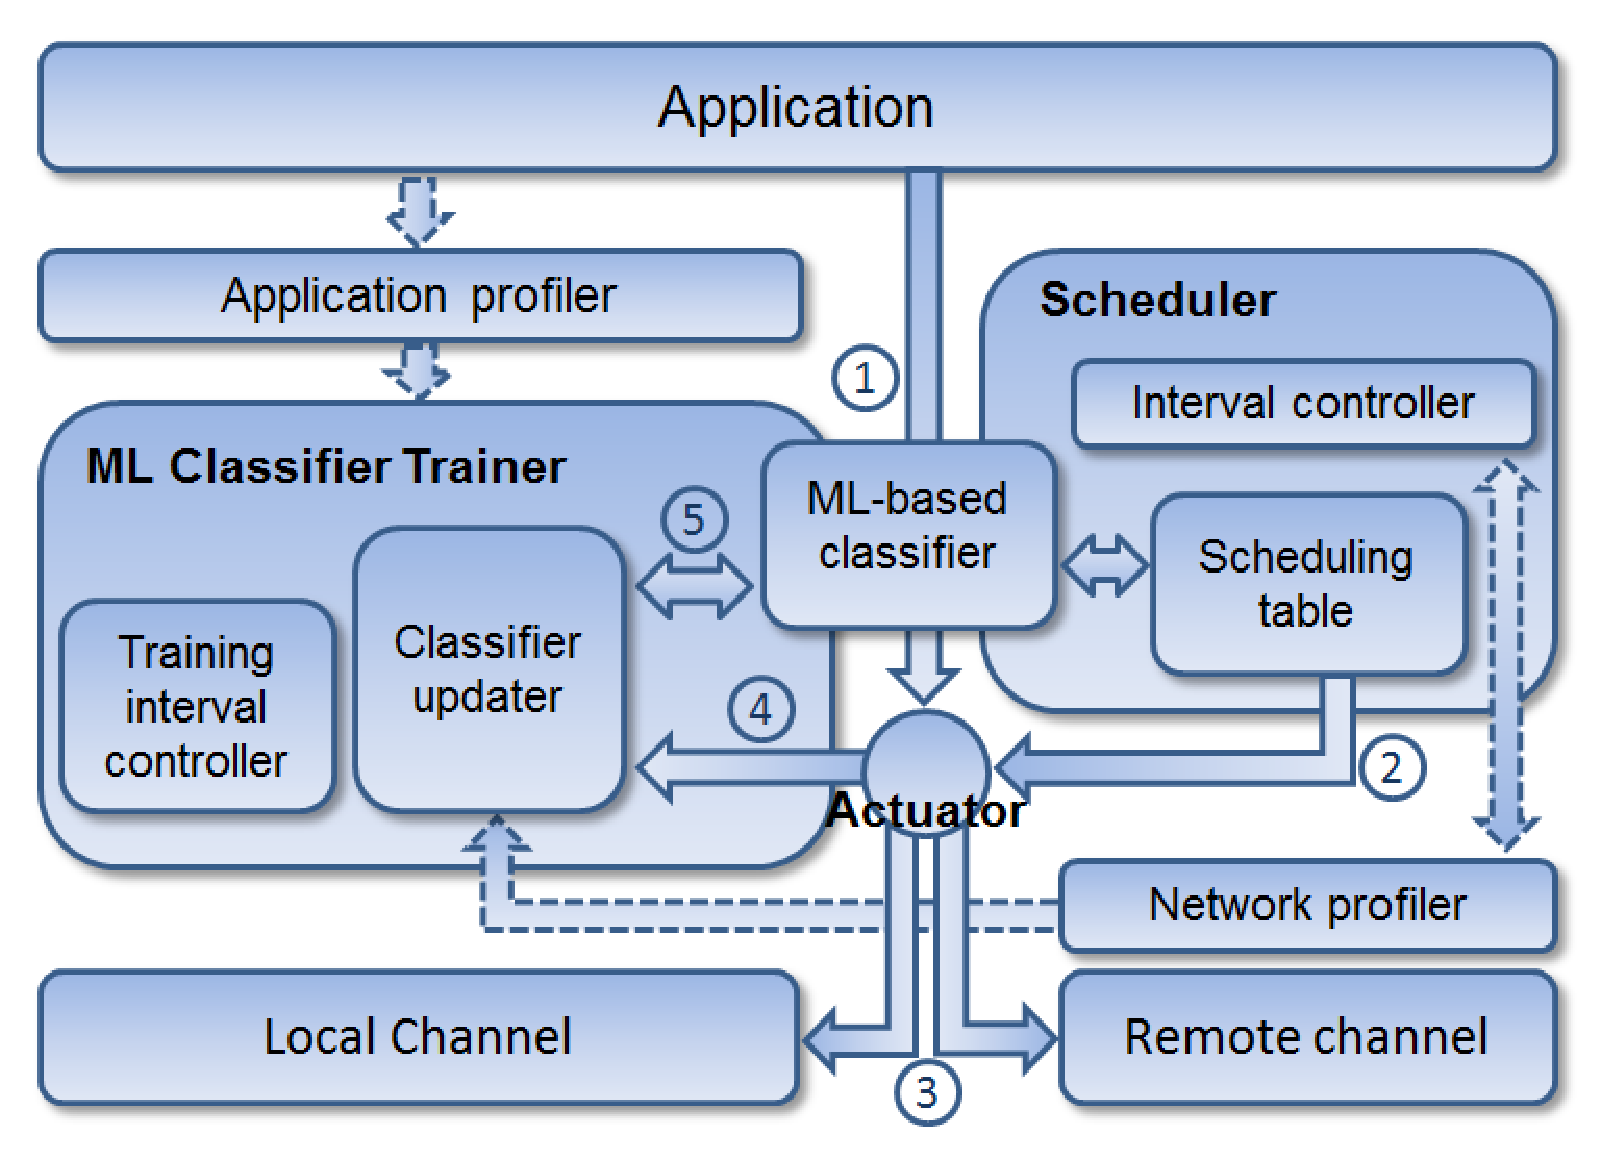
\includegraphics[height=5.1cm, width=7.6cm]{Figure/figure1}
\caption{Overall architecture of the ML-based mobile offloading
scheduler with online training. The dotted lines indicate the
application and network features flow path, and the solid lines are the
applciation workloads or scheduling-related commands flow path.}
\end{figure}
%
\subsection{Architecture of the Machine Learning-based Mobile Offloading
Scheduler}
%
As depicted in Figure 1, the overall architecture of the machine
learning-based mobile offloading scheduler with online training consists
of four main modules: computation router, runtime scheduler, machine
learning classifier, and machine learning classifier trainer which
interact with each other to execute and schedule the mobile computing
tasks, and train the machine learning classifier.\\
%
\textbf{Computation router.} The computation router has the
responsibility to route the mobile computing tasks either to the remote
channel (for offloading) or to the local channel (for local processing)
according to the scheduling table which stores the scheduling status of
each computing task.
%
Also, the router keeps the feedback channel with the classifer updater
in the machine learning classifier trainer module so that it provides
the performance comparison between offloading and local processing 
the offloading and local processing performance.\\
%
\textbf{Runtime scheduler.} Since scheduling mobile computations
requires to profile internal and external dynamic features which are
used for machine learning attributes such as data size and network
conditions on runtime, the scheduling process results in the additional
costs in terms of the execution delay and energy consumption.
%
Thus, there exists the tradeoff between the scheduling performance and
cost, as coarse-grained scheduling is much cheaper than frequent
scheduling, but it leads worse scheduling accuracy.    
%
For this reason, we consider two scheduling strategies.
%
First strategy reschedules the mobile computations whenever the
application executes these mobile computations.
%
We refer this strategy to the \textit{on-demand scheduling}.
%
Another strategy is the \textit{periodic scheduling} in which the mobile
computing tasks are rescheduled asynchronously with the adaptive
scheduling interval.
%
In the periodic scheduling strategy, in other words, scheduling the mobile
computations is done with the specific interval regardless of the
invocations of the mobile computations from the application.
%
However, in order to prevent unnecessarily too frequent scheduling, the
scheduling interval controller changes the scheduling interval according
to network conditions such that the interval becomes shorter if the
variation of network bandwidth is less than a certain threshold.
%
Otherwise, the scheduling frequency leaves in a long interval mode.
%
To end this, the scheduling interval controller stores previous
\textit{N} network bandwidth measurement histories.\\
%
\textbf{Machine learning classifier.} The machine learning classifier is
in charge of making decisions on offloading or local processing for the
offloadable mobile computing tasks by using the attributes obtained by
the network and application profiler.
%
Even though it is possible to adopt various attributes to capture the
present scheduling problem from internal and external environments, for
the current implementation, we utilized two attributes: the size of data
to be sent to the remote resource and network bandwidth.
%
It is also worth noting that, in the periodic scheduling mode, the
real-time measurement of the data size of the mobile computations is
unfeasible because the scheduling process is triggered periodically, but
asynchronously regardless of the invokations of the mobile computations.
%
In the periodic scheduling mode, instead, the application profiler
calculates the mean and standard deviation of the previous measurements
to anticipate the maximum and minimum possible data size.
%
Then, the machine learning classifier makes the decision on offloading
only when both classifications with the maximum and minimum possible
data size agree on offloading.\\
%
\textbf{Machine learning classifier trainer.} With the feedback on the
performance comparison between offloading and local processing from the
computation router, the machine learning classifier trainer updates
the machine leanring classifier.
%
In order to compare the performance between offloading and local
processing, the trainer creates one separate thread for local
processing, so that offloading and local processing can be executed
simultaneously.
%
Then the computation router measures the execution time for both
offloading and local processing to compare the performance and provide
the feedback into the classifier updater.
%
Finally, with this feedback from the computation router and the
attributes from the profilers, the classifier updater trains the
classifier.
%
\subsection{Adaptive Online Training Mechanism}
%
\begin{figure}
\centering
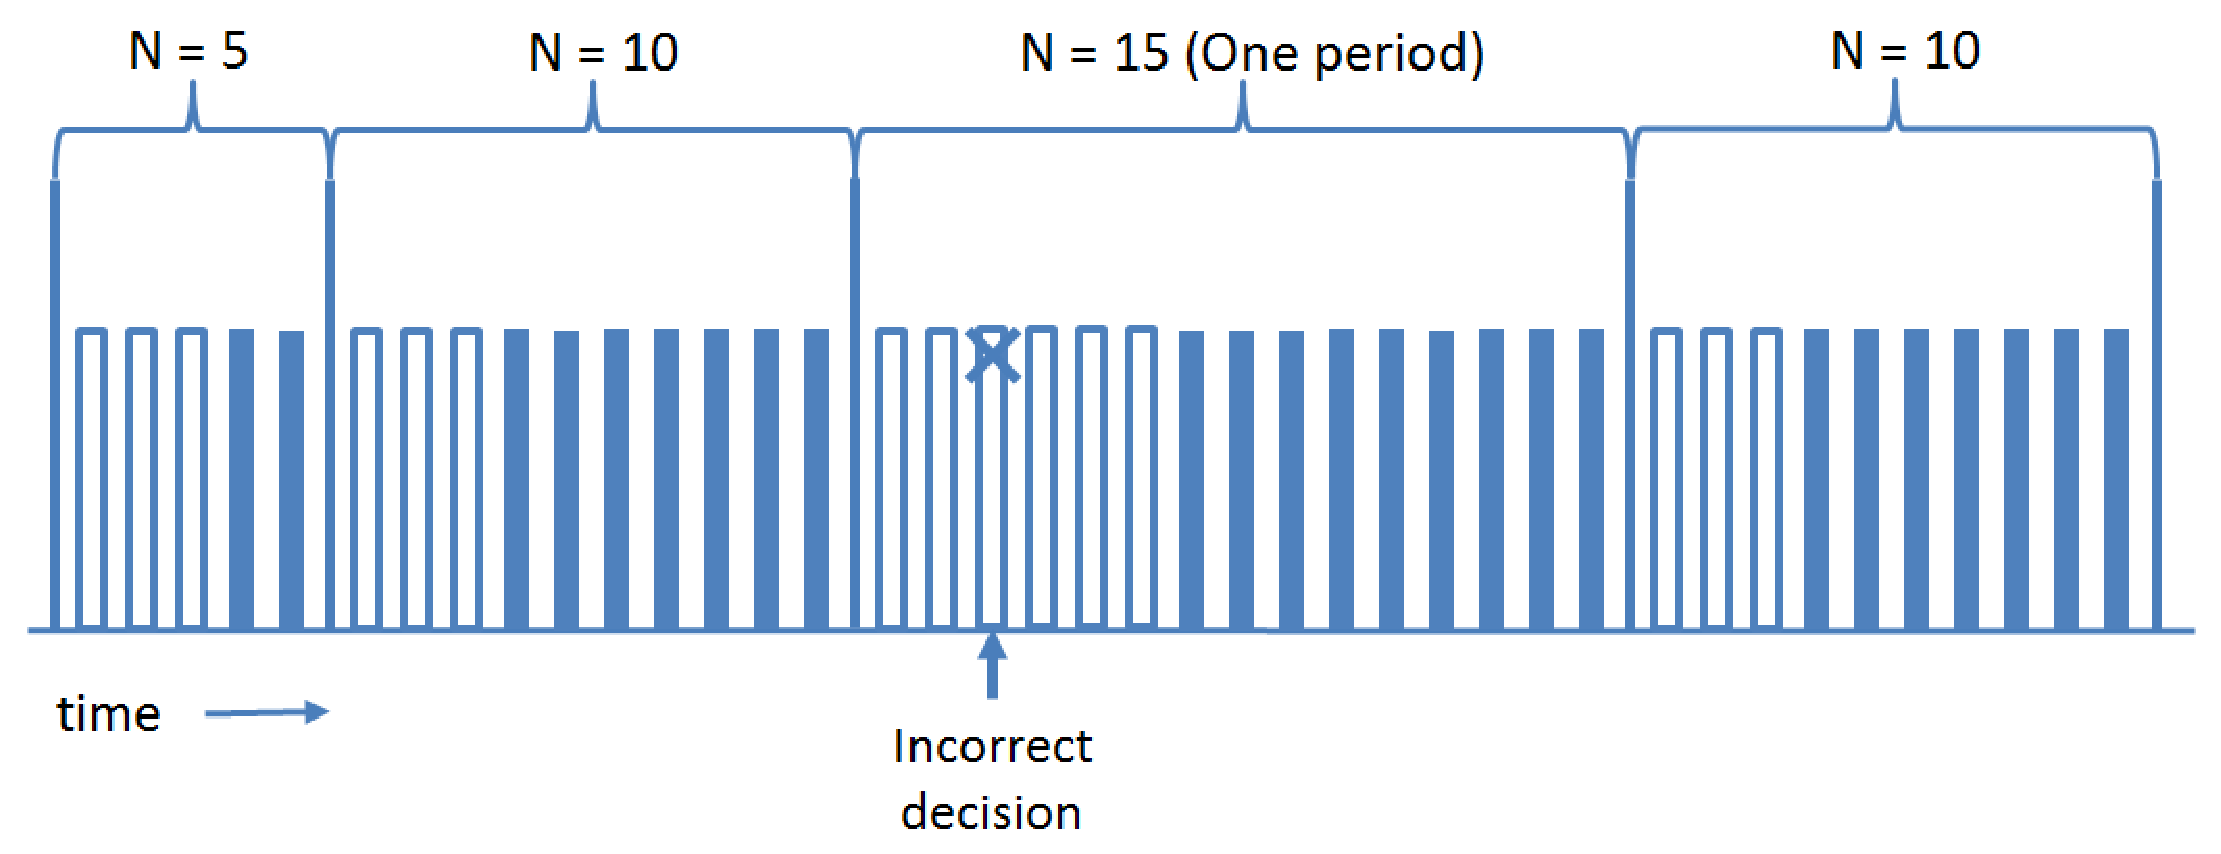
\includegraphics[height=3.3cm, width=8.5cm]{Figure/figure2}
\caption{An example of the adaptive online training mechanism. For this
example, we set 70\% of the scheduling accuracy threshold and 5 of the
minimum number of the mobile computation executions.}
\end{figure}
%
One of important contributions of this work is the adaptive online
training mechanism in which the training phase stretches and shrinks
according to the scheduling performance (i.e. scheduling accuracy).
%
Figure 2 illustrate the example of how the adaptive online training
mechanism.
%
In this example, we set the minimum number of the executions of the
mobile computations in one period to 5.
%
First of all, the training phase (empty bars) in a period
continues until the scheduling accuracy is higher than a certain
threshold.
%
In order to avoid 100\% of the scheduling accuracy at just one training,
we insert a dummy training which does nothing with the training process,
but indicates an incorrect decision. 
%
By adding this dummy training into the measurement of the scheduling
accuracy, more than one training in a period can be guaranteed.\\
%
\indent Once the training phase finishes, the normal operation phase
follows by starting the scheduling process until the period is
completed.
%
Since we set 70\% of the accuracy threshold for this example and no
decision error happened in the first and second period, the machine
learning can be trained for first three of executions and the rest of
the executions (two for the first period and seven for the second
period) are done in the normal operation phase. 
%
Furthermore, because there was no decision error in the first and second
period, the next number of the executions of the mobile computation
increases by 5 which is the minimum number of the executions in a
period, thus, the number of the computation executions for the second
and third period becomes 10 and 15 respectively.
%
In the second period, however, as one incorrect decision has been
occurred, the training phase holds for six executions when the
scheduling accuracy becomes higher than 70\%, and the number of the
executions in the fourth period decreases by 5 which is the minimum
number of the executions in a period multiplied by the number of the
occurred errors (in this case, 1). 
%
The pseudo-code of the adaptive online training mechanism is shown in
Figure 3.
%
\begin{figure}
\algsetup{indent=1.0cm}
\begin{algorithmic}[1]
\STATE{\textit{$//$ switch the training and normal operation phase}}
\WHILE{$one$ $period$ $is$ $NOT$ $finished$}
	\IF{$it$ $is$ $in$ $normal$ $operation$ $phase$}
		\STATE {$do$ $scheduling$}
	\ELSE
		\IF{$accu_{curr}$ $is$ $higher$ $than$ $th_{accu}$}
			\STATE{$switch$ $normal$ $operation$ $phase$}
		\ELSE
			\STATE{$stay$ $training$ $phase$}
		\ENDIF
	\ENDIF
\ENDWHILE
\STATE
\STATE{\textit{$//$ calculate the length of the next period}}
\IF{$errors$ $happened$}
	\STATE{$period_{next}$$\gets$$period_{curr}$$-$$($$period_{min}$$\times$$n_{err}$ $)$}
\ELSE
	\STATE{$period_{next}$$\gets$$period_{curr}$$+$$period_{min}$}
\ENDIF
\end{algorithmic}
\caption{Adaptive online training mechanism}
\end{figure}
%
\subsection{Integration with Mobile Offloading Framework}
%
As part of the modularization effort, we integrated the modules of the
machine learning-based mobile offloading scheduler into the Java-based
offloading-capable mobile applications which are automatically
refactored by a novel tool, called DPartner.
%
\section{Evaluation}
%
\subsection{Experimental Setup}
%
\subsection{Training Cost}
%
\subsection{Offloading Decision Performance}
%
\section{Use Case}
%
\section{Conclusion and Future Work}
% 
%\section*{Acknowledgement}
%This material is based upon work supported in part by the National Science
%Foundation under Grant No. 0910812, 0758596, 0855031, and 1265341.
%
%Any opinions, findings, and conclusions or recommendations expressed in
%this material are those of the author(s) and do not necessarily reflect
%the views of the National Science Foundation.
%
%\bibliographystyle{IEEEtran}
\bibliography{ipccc14}
\end{document}


